\documentclass[conference]{IEEEtran}
\IEEEoverridecommandlockouts
% The preceding line is only needed to identify funding in the first footnote. If that is unneeded, please comment it out.
\usepackage{cite}
\usepackage{amsmath,amssymb,amsfonts}
\usepackage{algorithmic}
\usepackage{graphicx}
\usepackage{textcomp}
\usepackage{xcolor}
\documentclass{article}

\usepackage{hyperref}
\usepackage{listings}
\usepackage{xcolor}

\definecolor{codegreen}{rgb}{0,0.6,0}
\definecolor{codegray}{rgb}{0.5,0.5,0.5}
\definecolor{codepurple}{rgb}{0.58,0,0.82}
\definecolor{backcolour}{rgb}{0.95,0.95,0.92}

\lstdefinestyle{mystyle}{
    backgroundcolor=\color{backcolour},   
    commentstyle=\color{codegreen},
    keywordstyle=\color{magenta},
    numberstyle=\tiny\color{codegray},
    stringstyle=\color{codepurple},
    basicstyle=\ttfamily\footnotesize,
    breakatwhitespace=false,         
    breaklines=true,                 
    captionpos=b,                    
    keepspaces=true,                 
    numbers=left,                    
    numbersep=-6pt,                  
    showspaces=false,                
    showstringspaces=false,
    showtabs=false,                  
    tabsize=2
}

\lstset{style=mystyle}

\def\BibTeX{{\rm B\kern-.05em{\sc i\kern-.025em b}\kern-.08em
    T\kern-.1667em\lower.7ex\hbox{E}\kern-.125emX}}
\begin{document}

\title{Geomedia: a framework to share comments and multi-media content based on location.\\
{\footnotesize \textsuperscript{*}Project of "Wireless Network for Mobile Application", Master Degree in Computer Science at University of Padua}
}

\author{\IEEEauthorblockN{ Prof. Claudio Enrico Palazzi}
\IEEEauthorblockA{\textit{Department of Mathematics} \\
\textit{University of Padua}\\
Padua, Italy \\
cpalazzi@math.unipd.it}
\and
\IEEEauthorblockN{ Alberto Morini}
\IEEEauthorblockA{\textit{Department of Mathematics} \\
\textit{University of Padua}\\
Padua, Italy \\
alberto.morini@studenti.unipd.it}
}

\maketitle

\begin{abstract}
Nowadays Social Networks are the principal way to create connections among people.
Platforms like Facebook, Twitter, and Instagram offer users content and profiles based not only on mutual connections and trending content but also on geographic location.
\\
GeoMedia is a framework, developed into an Android Application, which provide a medium for users to share comments and multimedia content (such as photos, videos, and audio) based on their location.
Then, users can easily see the content shared through GeoMedia moving across a geographical map.
\end{abstract}

\begin{IEEEkeywords}
Android, Social Networks, user location, privacy, client server, multimedia, media sharing, android location, http, three-tier, three-tier architecture, SQL, DBMS
\end{IEEEkeywords}

\section{Introduction}
In the last decade, mobile applications has almost replaced traditional computer programs, especially when comes to social networks. Not only because it is more convenient to use a mobile phone than a laptop, but also because mobile phones can give more functionality by using physical sensors to enrich the user experience.


The explosion of social media led media companies to invest and explore almost all functionality of the mobile device, thus to make users feel more connected and satisfied by providing more relevant content. As a result, users spend more time on these platforms, generating profit for social media companies.
A perfect example is Tinder, a dating app where users can meet each other based on their geographical proximity.
\\
For reach this purpose, a variety of sensors can be used to profile the end user, often using the GPS to get the precise location, otherwise opting to the proximal location provided by Access Point / Cell antenna.

However, utilizing these features can lead to faster battery drain, higher data usage, and potential privacy concerns.
\\
This project aims to develop a mobile application that allows users to share comments, photos, audio, videos, and other multimedia content on where they are, and then, see the content through a map.

\section{Architecture}


To ensure that the GeoMedia app functions as intended, there's the need to design an opportune architecture, event if not strictly related with the application itself; the "three-tier" model adopted, will allows mobile apps to communicate each other without a direct connection.

\begin{figure}[htbp]
{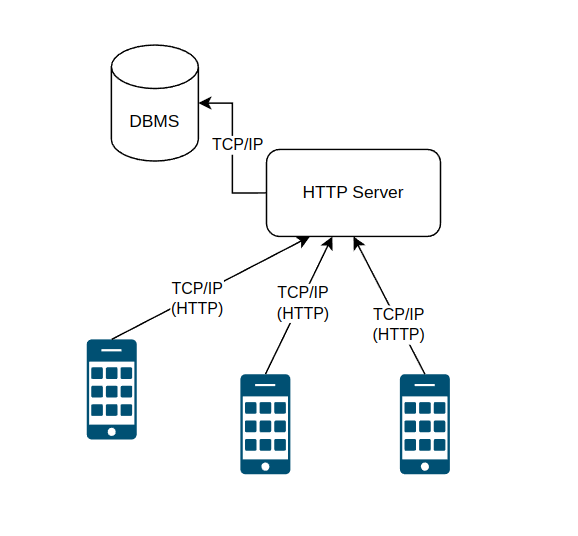
\includegraphics[width=9.5cm]{imgs/Architecture.png}}
\caption{Design Architecture.}
\label{fig}
\end{figure}

\subsection{Presentation layer}
The presentation layer consists of the "GeoMedia" app itself, acting as the interface between the users and the data stored on the servers (by the application and data layers). Users will interact with the mobile application to view others' posts or share their own content.
In the last case, this layer is for retrieving necessary data, such as the user's location, user identifier (username), and others metadata.

\subsection{Application layer}

In this project, the application layer is represented by an HTTP server, which exposes endpoints to the frontend (presentation layer) and then process the requests received.
\\
Specifically, for each endpoint, server will manipulate data with opportune SQL instruction through the Data Layer.

\subsection{Data layer}

The Data Layer consists of a Database Management System (DBMS), capable of performing CRUD operations (Create, Read, Update, Delete) on data stored in well defined tables.
\\
For this project, the DBMS will also be used to create SQL stored procedures, thus to offer to development a more flexible way to modify the select or insert of data queries.


\section{Mobile application}
In way to create a mobile application there are several frameworks and technologies options. For this project has been selected the "Ionic Framework" \cite{b1}, an open source toolkit for building cross-platform mobile, web, and desktop applications using web technologies such as HTML, CSS, and JavaScript.
One of the key advantages of the Ionic Framework is its ability to integrate  web frameworks such as ReactJS, that offers a major benefit: it efficiently updates the DOM by re-rendering only those components that have changed, preventing unnecessary updates to unchanged elements.\\
React.js also expose some "hooks" where can be injected the call for personalized functions, thust to execute the code whenever the users interact with the app.
For example, hooks like useEffect() and useState() respectively allows to call functions at the component startup or when a property change, giving to the development the ease of personalization.
\\
As follow an example of a React Component created
\begin{lstlisting}[language=Java, caption=Map component snippet]
//various imports ...
import { useContext, useEffect, useState } from "react";
const MyPMap = () => { //declare the Map component

    const [PostList, setPostList] = useState([]) //to store the list of posts
    const ctx = useContext(mycontext)  //use the React context to retrieve data of other components
    
    // retrieve all post giving the actual position of user (in the server it will be computed the nearest posts)
    function getPosts() {
        if (ctx?.UserPosition != null) {
            doRequest("getPosts", {
                latitude: ctx?.UserPosition[0]
                , longitude: ctx?.UserPosition[1]
            }).then(res => {
                setPostList(res)
            })
        } else {
            doRequest("getPosts", {
                latitude: null
                , longitude: null
            }).then(res => {
                setPostList(res)
            })

        }
    }
    
    useEffect(() => {
        getPosts(); //to call the post
    }, []); //at the startup of component
    return( //render the graphics
        <>
        <Map defaultCenter={ctx?.UserPosition} defaultZoom={11}>
            <ZoomControl />
            <Marker width={50} anchor={ctx?.UserPosition} color={"#154c79"} />
            {
                PostList?.map(s => (
                    <Marker width={50} anchor={[s.LATITUDE, s.LONGITUDE]} color={(s?.MEDIATYPE?.length > 0) ? '#d6c531' : '#f23c3c'}
                        onClick={() => {
                            setPostSelected(s) //store the post selected to open it in the opportuned component (viewPost)
                        }}
                    />
                ))
            }
        </Map>
        ...
        </>
    );
}
export default MyPMap;
\end{lstlisting}

\begin{figure}[htbp]
\begin{center}
{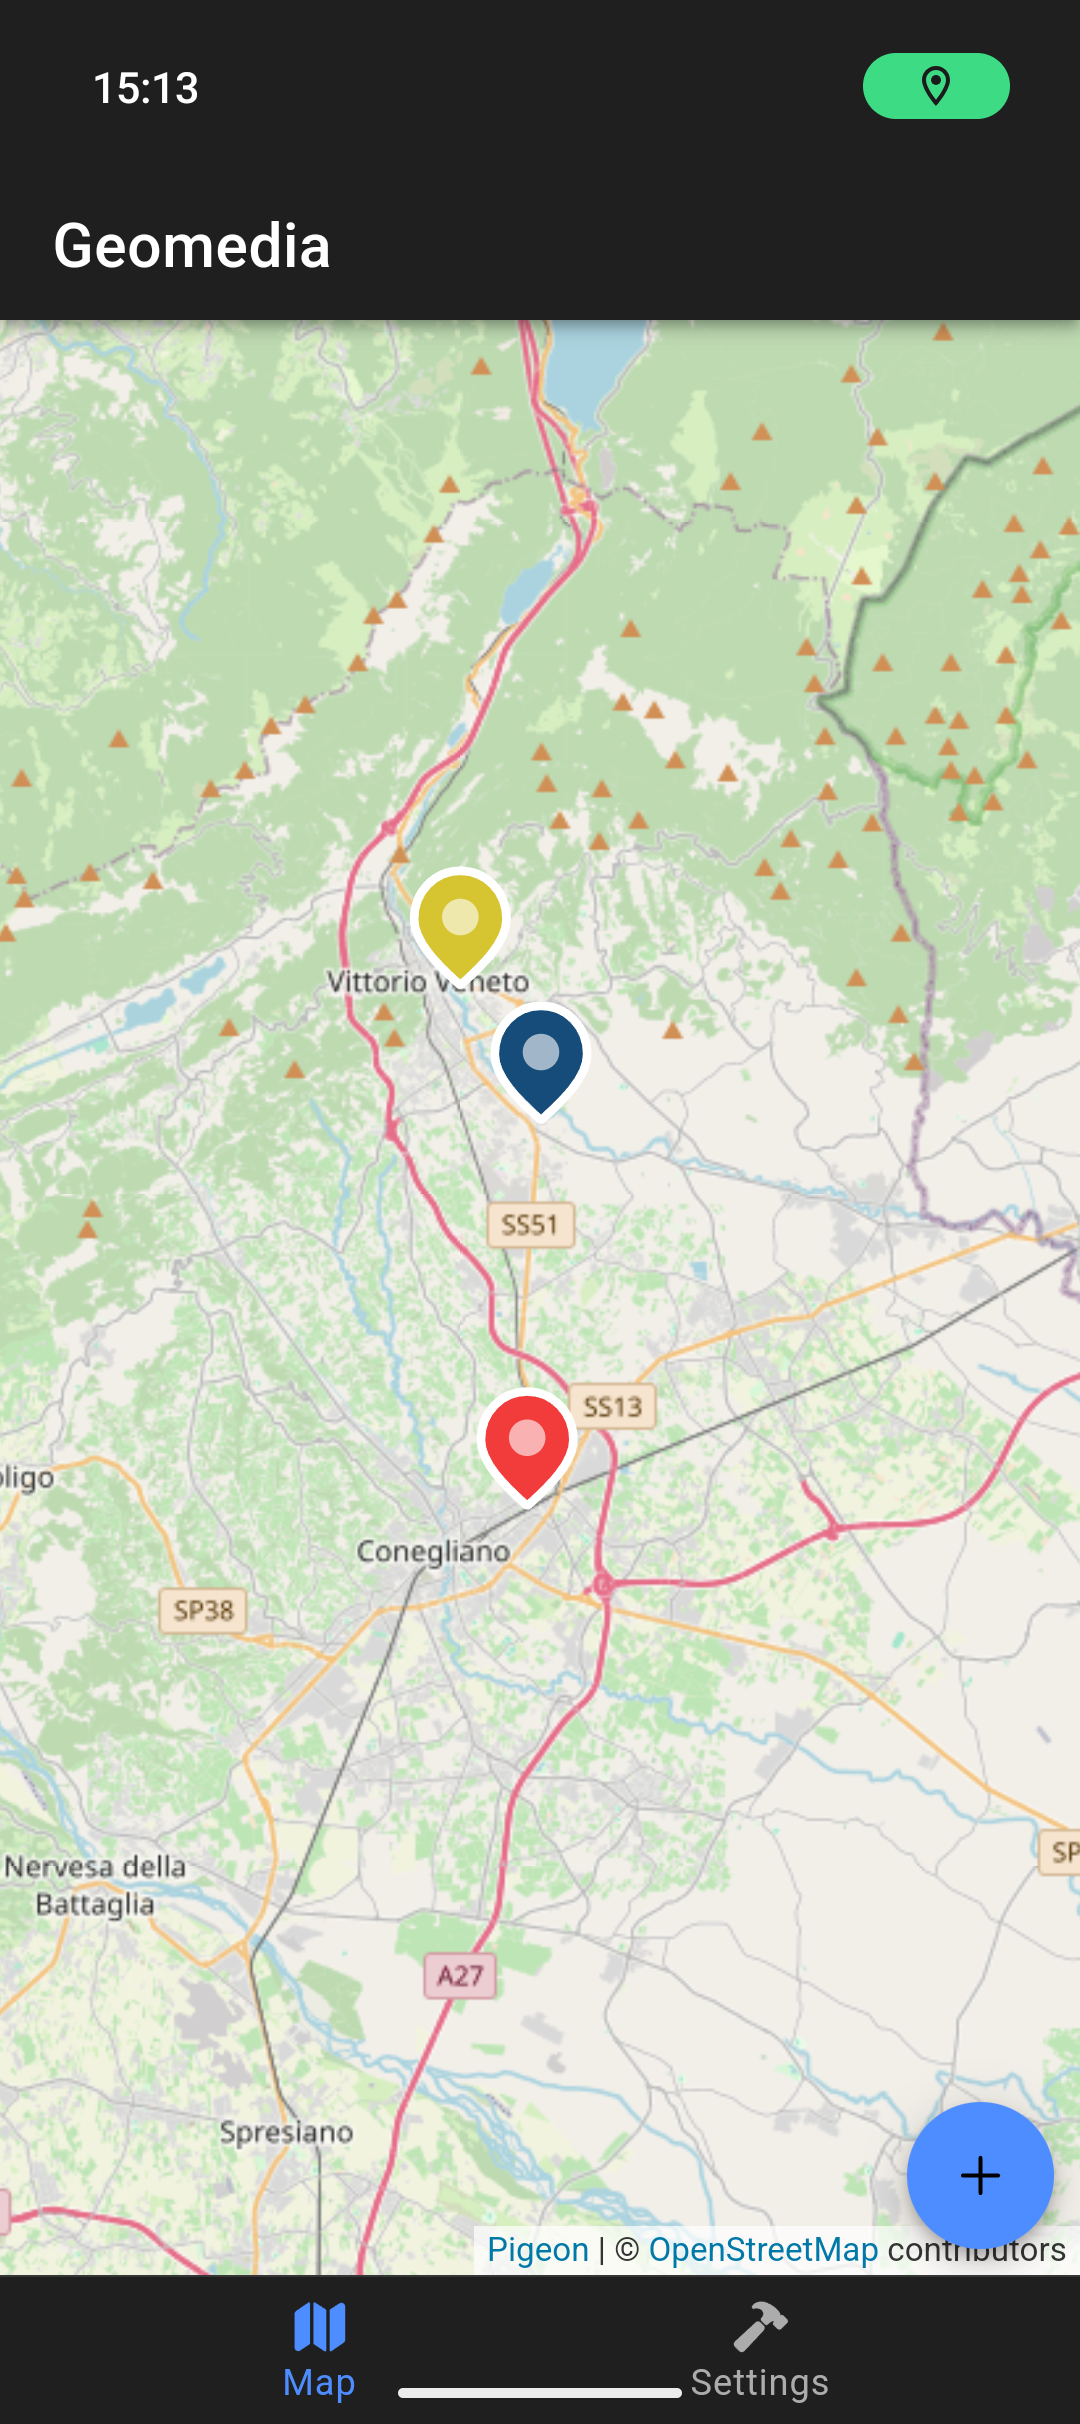
\includegraphics[width=5.5cm, height=11cm]{imgs/Map.png}}
\end{center}
\caption{Example of Map component.}
\label{fig}
\end{figure}


In the React component declared, has been used also the Pigeon Map\cite{b8} as React Component, which renders a geographical map and consents to put some 'marker'.
In GeoMedia, there are three types of markers.
\begin{itemize}
\item Blue marker: the current user location
\item Red marker: a post with just text (comment)
\item Yellow marker: a post with a media attached 
\end{itemize}

At the startup of the component (triggered after the user login), an HTTP request is made to the server to retrieve the posts previously uploaded in GeoMedia, then each post will be rendered as market on the map.
\\
The method is parameterized to get all posts, or to make the server compute the post closer to the location provided within a defined range.
This strategy is can be useful for scenarios like events or game-plays, where users need to be  within a certain area to access exclusive data.


Another key component is 'ViewPost.jsx', which serves the purpose to show the comment of the clicked market, by opening a new interface and fetching the server to retrieve any associated multimedia data.
This component is not limited to just viewing the comment; it also provides the functionality for downloading the attached multimedia file and store into the local storage of the mobile.



\begin{lstlisting}[language=Java, caption=ViewPost]
const ViewPost = (props) => {
     const refModalPost = useRef()
    const ctx = useContext(mycontext)
    const [DataBase64, setDataBase64] = useState(null) //to store the mediafile attached

    async function downloadFile(file) {
        let checkPer = await Filesystem.checkPermissions()
        let ask = await Filesystem.requestPermissions()
        try {
            let y = await Filesystem.writeFile({
                path: file.MEDIAFILENAME,
                data: DataBase64,
                directory: Directory.Documents,
            });
            if (y.uri.length > 0) {
                ctx?.showMessage("File saved into Documents folder", "success")
            }
        } catch (error) {
            alert(error)
        }
    }
     // get the media content in base64, different endpoint due to increment performance
    function getMediaPost(postid) {
        doRequest("getMediaPost", {
            POSTID: postid
        }).then(res => {
            //res[0]?.MEDIADATA
            if (res[0]?.MEDIADATA != null) {
                setDataBase64(res[0]?.MEDIADATA)
            }
        })
    }
    return(
    <>
        <IonModal>
        </IonModal>
    </>
    )
}
\end{lstlisting}


\begin{figure}[htbp]
\begin{center}
{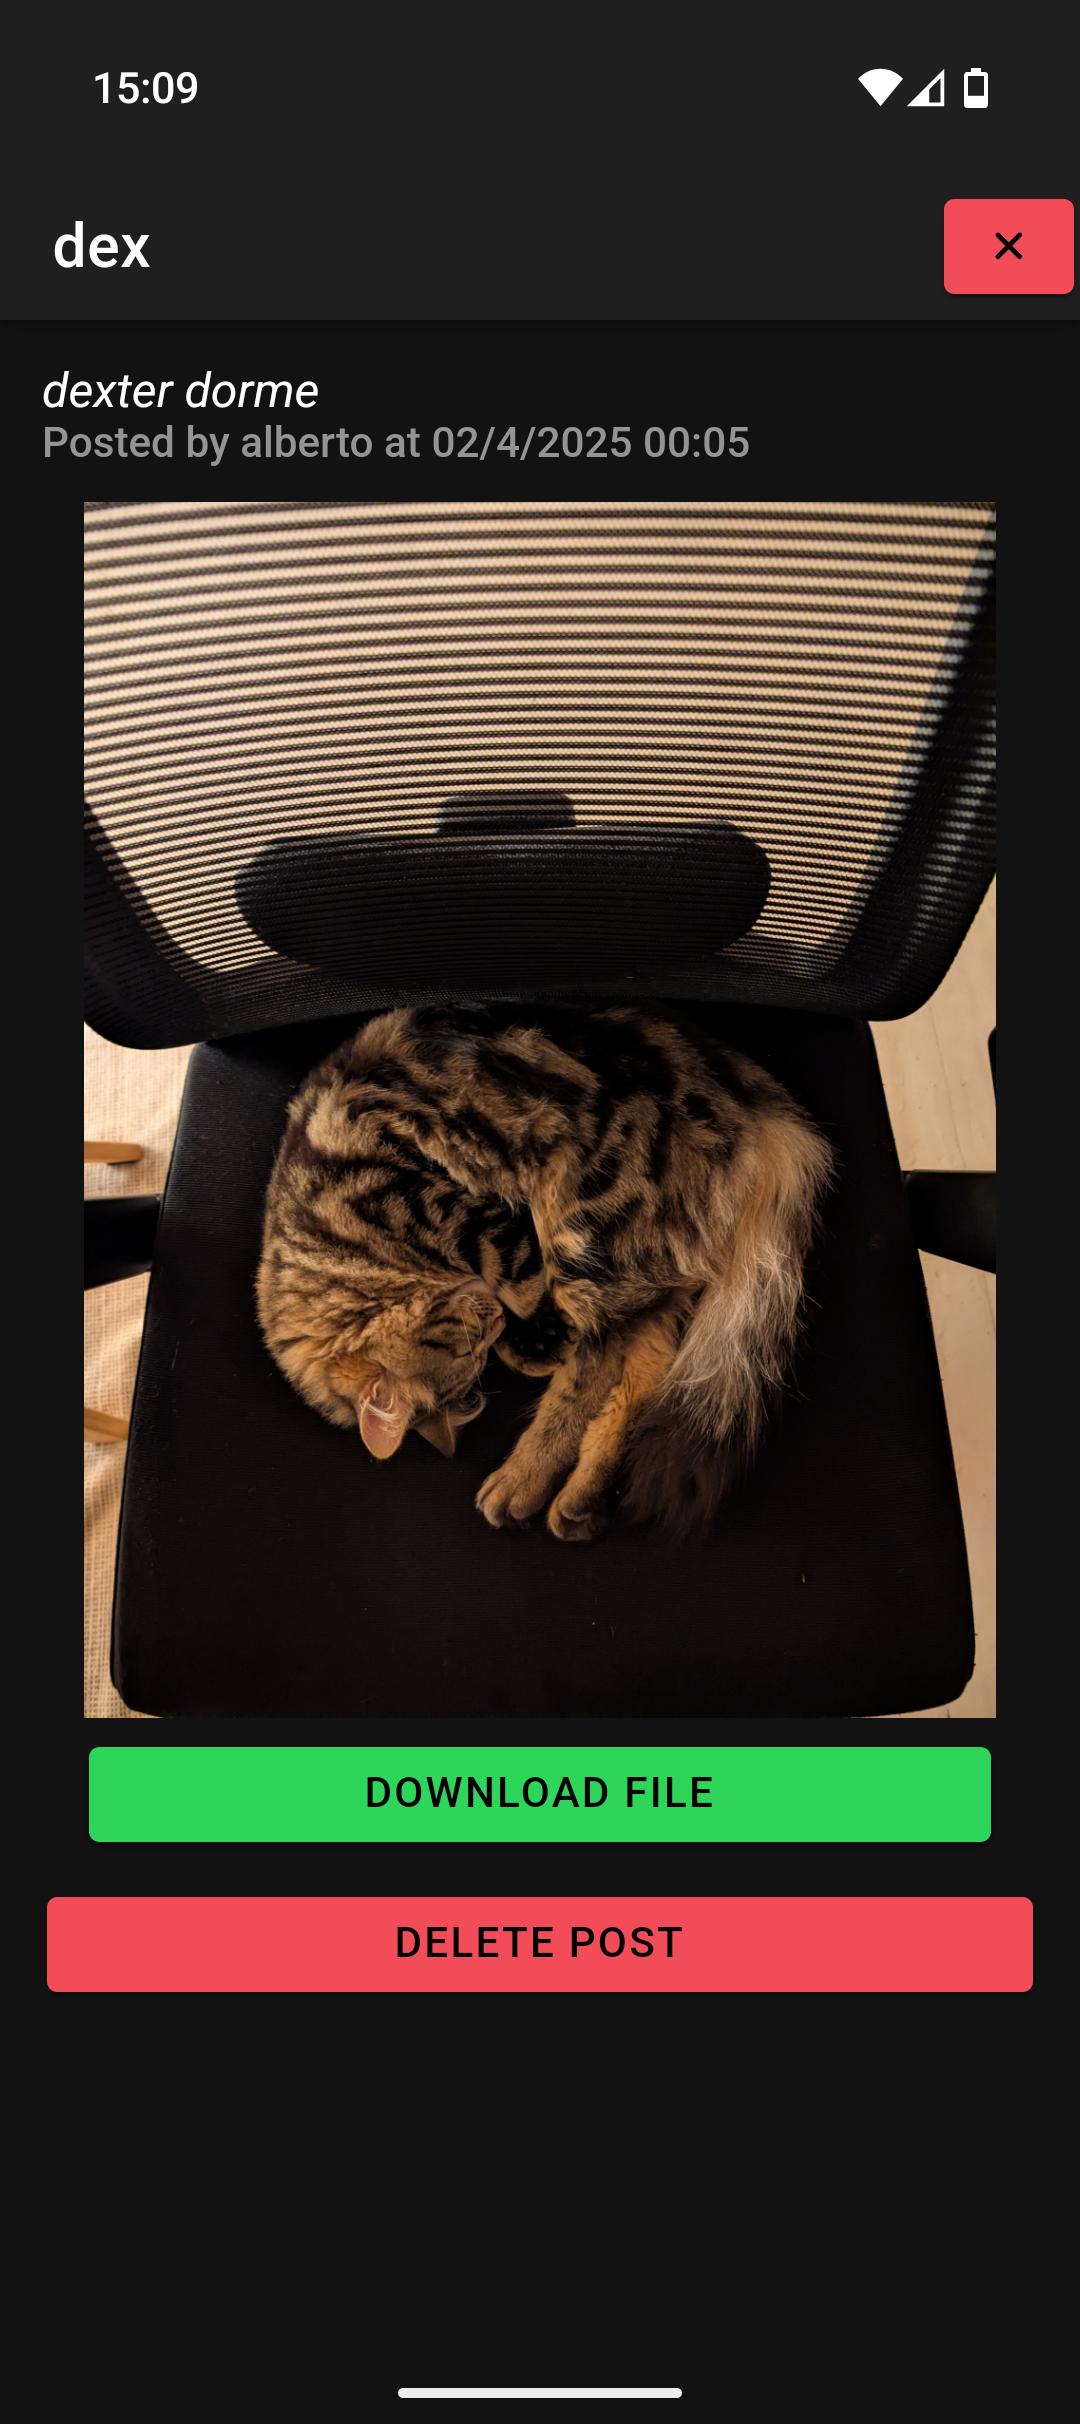
\includegraphics[width=5.5cm, height=11cm]{imgs/PostView.png}}
\end{center}
\caption{Example of Post view.}
\label{fig}
\end{figure}


\subsection{Ionic Capacitor}

In order to access physical sensors on Android, such as geolocation and file storage, Ionic Capacitor can be integrated into the Ionic Framework. Capacitor is a collection of libraries that make possible the integration of web applications with native components, providing the API to adopt at Javascript level.

Geomedia require to use some defined modules of capacitor, in specific:
\begin{itemize}
    \item GeoLocation\cite{b2}: to get latitude and longitude coordinate of user logged into the app
    \item FileSystem\cite{b3}: to store file into mobile filesystem whenever users want to download the media uploaded
\end{itemize}

These plugins can be installed via a shell command, respectively:
\begin{itemize}
    \item `\$ npm install @capacitor/geolocation`
    \item `\$ npm install @capacitor/filesystem'
\end{itemize}

The geolocation package provide the method `getCurrentPosition()` which returns an Object with parameters like: latitude, longitude, altitude and accuracy for each type of coordinate. The altitude even if not relevant for this project, could be integrated in future development thus to create more peculiar scenario or use cases.


\subsection{Building for Android}

A key strength of the Ionic Framework is its ability to build web applications into native mobile apps; in fact the framework acts as a wrapper/interpreter for the webpage, essentially embedding a custom browser inside the app.
\\
To create an Android Package (APK) for installing the app, some shell commands are required as reported in the official documentation, such as:
\begin{itemize}
    \item 'npm install @capacitor/android' to add the capacitor
    \item  'npx cap add android' to denote the android platform, since Ionic can also build for "iOS" operating system
    \item 'npx cap build android' to export the application in production mode and so encapsulate the app into a bundle that later will be compiled
\end{itemize}


At this point some modification to the Android Manifest are required thus to declare the necessary permissions and other metadata.
Specifically, to access the user's geolocation, GeoMedia requires the user to grant permission due to privacy purposes.
\\
Another modification is to allow clear traffic (HTTP), since from Android 8, only HTTPS packets are allowed by default unless the explicitly declaration in the manifest.

\begin{lstlisting}[language=XML, caption=Snippet of Android Manifest]
<application
    android:allowBackup="true"
    android:icon="@mipmap/mymap"
    android:label="@string/app_name"
    android:roundIcon="@mipmap/mymap_round"
    android:supportsRtl="true"
    android:requestLegacyExternalStorage="true"
    android:largeHeap="true"
    android:usesCleartextTraffic="true"
>
...
</application>
...
<uses-permission android:name="android.permission.ACCESS_COARSE_LOCATION" />
<uses-permission android:name="android.permission.ACCESS_FINE_LOCATION" />
<uses-feature android:name="android.hardware.location.gps" />
        
\end{lstlisting}

\section{HTTP Server}

In the application layer the HTTP server takes place, which represent the bridge between data stored and the mobile application explained before.
The GeoMedia HTTP server use NodeJS\cite{b4} as engine to start a listening process on a designated network port; even more, the server exposes several path called endpoints, each corrisponde to a specific function within the application. In fact, the server map the request to the execution command of a SQL stored procedure, which handles the designed queries on the respectively tables.

The package handled in this platform has a content-type of JSON (JavaScript Object Notation) thus to allow a rapid extendability of data included and providing an easily human-readable format.
Only the "POST" method is implemented, since every request/response include data and parameters.

The server requires just one external dependency not included natively, which is 'tedious'\cite{b5} (installable via `\$ npm install tedious`) a module to establish a connection to Microsoft SQL Database (DBMS) then execute query commands and transactions.

\begin{lstlisting}[language=Java, caption=Snippet of GeoMedia HTTP server]
const http = require("http");
const port = 9911

/**
 * Invia una risposta HTTP
 * @param {Object} res res of http 
 * @param {int} status of response 
 * @param {Object} body 
 * @param {String} mime 
 */
function sendResponse(res, status, body = null, mime = "application/json") {
    res.writeHead(status, { 'Content-Type': mime, "Access-Control-Allow-Origin": "*" });
    try {
        if (mime == "application/json") {
            res.write(JSON.stringify(body));
        } else {
            res.write(body)
        }
    } catch (err) {
        res.write(err);
    }
    res.end();
}
http.createServer((req, res) => {
    let body = "";
    req.on("data", (chunk) => {
        body += chunk
    });

    req.on("end", () => {
        try {
            body = JSON.parse(body)
        } catch (error) {
            //nthg
        }
         if(req.url=="/checkConnection"){ // uitility, client on startup send this request, to make sure its configuratin is correct. If server responds the configuration is right
            sendResponse(res,200,{"HELLO":"From server!"})
        }

        try {
            switch (req.url) {
                case "/doLogin": //LOGIN OR REGISTER
                    dispatcher.doLogin(body.username, body.password, body.newuser).then(resQuery => {
                        sendResponse(res, 200, resQuery)
                    }).catch(err => {
                        sendResponse(res, 500, err)
                    })
                    break;
                case "/newPost":
                    dispatcher.newPost(body.author,body.postcontent).then(resQuery=>{
                        sendResponse(res,200,resQuery)
                    }).catch(err=>{
                        sendResponse(res,500,err)
                    })
                    break
               case "/getPosts":
                    dispatcher.getPosts(body?.LATITUDE, body?.LONGITUDE,body?.USERNAME).then(resQuery=>{
                        sendResponse(res,200,resQuery)
                    }).catch(err=>{
                        sendResponse(res,500,err)
                    })
                    break
                ...
                default:
                    sendResponse(res, 404, { 'msg': "Unknown path:" + req.url })
                    break;
            }
        } catch (error) {
            fs.appendFileSync('./log.txt', 'ERROR ,' + Date.now() + ',' + error)
        }

    })
}).listen(port);

console.log("Server started on port: "+port);

\end{lstlisting}


The server represent a single access point, which is a fragile solution in a real-world scenario, as it represents a "single point of failure" where the failure of a this node makes unavailable the whole system.
\\
There are many alternatives to mitigate this event. One approach is to replicate the HTTP server across different machines, introducing the challenge of synchronizing multiple main servers.
A more sophisticated solution, is to change the whole design of this solution, creating a distributed architecture by adopting microservices\cite{b6}; where the server is fragmented into multiple smaller process that acts one for each specific function.
For example, one microservice could handle the retrieving process of the posts, another could manage the accoutns, another the post creation, and so on. This approach not only imrpoves reliability but also helps to distribute traffic loads thust to prevening the system from an overwhelmed; a common problem with social media platforms when a mass requests (of viral contents) happens causing the "break the internet" effect.


\begin{figure}[htbp]
\begin{center}
{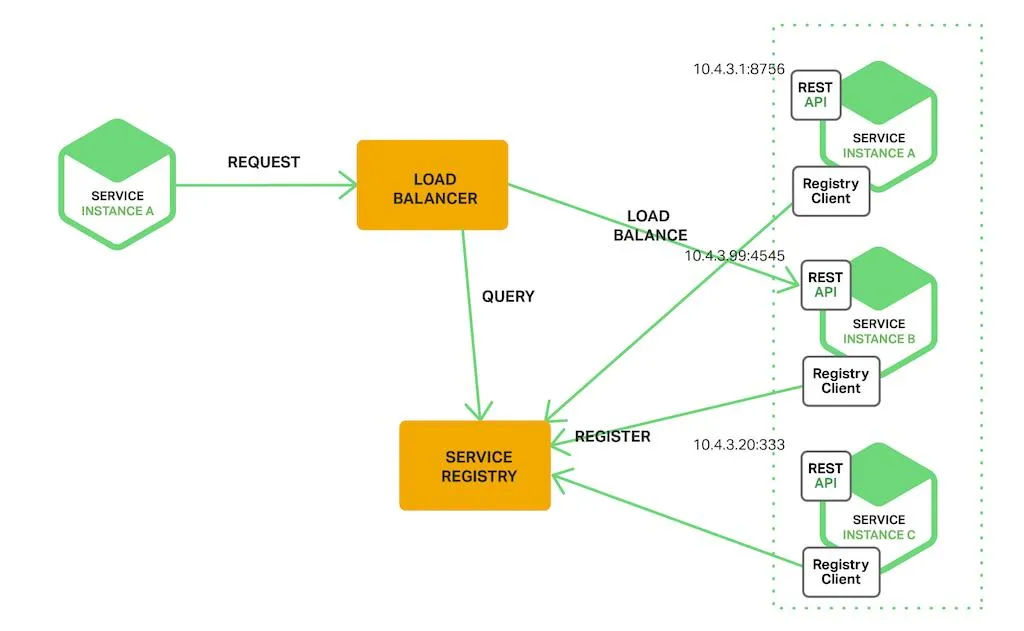
\includegraphics[width=10.5cm, height=7cm]{imgs/microservices.png}}
\end{center}
\caption{Example of Map component.}
\label{fig}
\end{figure}

\section{DBMS}

All posts published on GeoMedia are stored in a Database Management System (DBMS), where Microsoft SQL Server\cite{b7} serving as the engine.

The DBMS stores data in two primary tables:

\begin{itemize}
    \item `USERS` for users' profiles
    \item `POSTS` for posts 
\end{itemize}

\begin{lstlisting}[language=SQL, description=Creation of tables]
CREATE TABLE USERS(
    ID INT IDENTITY,
    USERNAME VARCHAR(50) PRIMARY KEY,
    PASSWORD NVARCHAR(256) NOT NULL, --stored the hash of MD5 function
);
CREATE TABLE POSTS(
	ID INT IDENTITY PRIMARY KEY,
	AUTHOR VARCHAR(50) FOREIGN KEY REFERENCES USERS(USERNAME),
	TITLE VARCHAR(50),
	COMMENT VARCHAR(MAX),
	MEDIATYPE VARCHAR(100), -- IMAGE/JPG, AUDIO/M4A
	MEDIADATA NVARCHAR(MAX), --BASE64
	POSTDATETIME DATETIME,
	COORD_X FLOAT,
	COORD_Y FLOAT,
);
\end{lstlisting}

Data is managed through stored procedures, which allows more efficient and accurate query modifications. For example, when storing a post,
the author (user) of the post and all associated metadata (as the whole JSON data received by server) are passed as parameters, then manipulated and formatted into SQL. Giving also the isolation and independence from the application layer.

\begin{lstlisting}[language=SQL, description=Stored Procedure of post creation]
CREATE PROCEDURE NEWPOST
@AUTHOR VARCHAR(50), @POSTCONTENT NVARCHAR(MAX)
AS
BEGIN
	
	INSERT INTO POSTS(AUTHOR,TITLE,COMMENT,MEDIATYPE,MEDIADATA,POSTDATETIME, LATITUDE, LONGITUDE)
	SELECT @AUTHOR, JJ.title, JJ.comment, JJ.mediatype, JJ.media_b64,GETDATE(), JJ.latitude ,JJ.longitude 
	FROM OPENJSON(@POSTCONTENT,'$') WITH(
		title  VARCHAR(50),
		comment  VARCHAR(MAX),
		media_b64  NVARCHAR(MAX),
		mediatype  VARCHAR(100),
		latitude FLOAT,
		longitude FLOAT
	) JJ
	
END;

\end{lstlisting}


\section{Future extensions}

In conclusion, GeoMedia offers a simple platform for sharing content on a geographic map. As previously mentioned, there are some key features that could be expanded.

Some ideas include:

\subsection{Live comments}
A potential feature to temporize posts to be available only at specific times or within a defined geographic area.
This could be used to create interactive experiences, such as "treasure hunts" or "hide and seek" games.

\subsection{Time capsule}

Extending the concept of limiting content to a specific area, another idea could involve storing posts in small sensors distributed randomly in locations such as forests, mountains, or cities. 
These sensors would be reachable only with short-range medium like Bluetooth or Wi-Fi, or even NFC.
\\
This idea could serve in multiple scenarios, such as a waypoints to mark hiking routes in the mountains, or actingas time capsules at panoramic points.


\begin{thebibliography}{00}
\bibitem{b1} Ionic Framework is cross-platform framework to create web-application and export them to mobile platform. \href{http://www.overleaf.com}{Link}
\bibitem{b2} Ionic Capacitor - Geolocation package to access to GPS location on mobile devices\href{https://capacitorjs.com/docs/apis/geolocation}{Link}
\bibitem{b3}Ionic Capactor - FileSystem package to store data on mobile devices\href{https://capacitorjs.com/docs/apis/filesystem}{Link}
\bibitem{b4} NodeJS as server engine \href{https://nodejs.org/en}{Link}\
\bibitem{b5}{Tedious - Node Package able to handle SQL Server communication} \href{https://tediousjs.github.io/tedious/}{Link}
\bibitem{b6} Microservices panoramic and image in figure \href{https://medium.com/the-modern-scientist/introduction-to-microservices-architecture-f0c7eefe79f1}{Link}
\bibitem{b7} Microsoft SQL Server 2022 as DBMSQ for data layer \href{https://www.microsoft.com/en-us/sql-server/sql-server-2022}{Link}
\bibitem{b8} Pigeon Map as React Component to render a geographical map \href{https://pigeon-maps.js.org/}{Link}


\end{thebibliography}
\vspace{12pt}

\end{document}
